% This must be in the first 5 lines to tell arXiv to use pdfLaTeX, which is strongly recommended.
\pdfoutput=1
% In particular, the hyperref package requires pdfLaTeX in order to break URLs across lines.

\documentclass[11pt]{article}

% Remove the "review" option to generate the final version.
\usepackage{acl}

% Standard package includes
\usepackage{times}
\usepackage{latexsym}

% For proper rendering and hyphenation of words containing Latin characters (including in bib files)
\usepackage[T1]{fontenc}
% For Vietnamese characters
% \usepackage[T5]{fontenc}
% See https://www.latex-project.org/help/documentation/encguide.pdf for other character sets

% This assumes your files are encoded as UTF8
\usepackage[utf8]{inputenc}

% This is not strictly necessary, and may be commented out,
% but it will improve the layout of the manuscript,
% and will typically save some space.
\usepackage{microtype}

% If the title and author information does not fit in the area allocated, uncomment the following
%
%\setlength\titlebox{<dim>}
%
% and set <dim> to something 5cm or larger.

\usepackage{graphicx}
\graphicspath{{../images/}}
\usepackage{booktabs}

\title{Testing Egunean Behin Visual Question Answering Dataset with BLIP}

% Author information can be set in various styles:
% For several authors from the same institution:
% \author{Author 1 \and ... \and Author n \\
%         Address line \\ ... \\ Address line}
% if the names do not fit well on one line use
%         Author 1 \\ {\bf Author 2} \\ ... \\ {\bf Author n} \\
% For authors from different institutions:
% \author{Author 1 \\ Address line \\  ... \\ Address line
%         \And  ... \And
%         Author n \\ Address line \\ ... \\ Address line}
% To start a seperate ``row'' of authors use \AND, as in
% \author{Author 1 \\ Address line \\  ... \\ Address line
%         \AND
%         Author 2 \\ Address line \\ ... \\ Address line \And
%         Author 3 \\ Address line \\ ... \\ Address line}

\author{Julen Etxaniz \\
  University of the Basque Country (UPV/EHU) \\
  \texttt{jetxaniz007@ikasle.ehu.eus}}

\begin{document}
\maketitle
\begin{abstract}
Egunean Behin is a new visual question answering dataset based on Egunean Behin game. It consists of three types of questions from the game: figures, cubes and maze. Questions require counting figures, colors, cubes and understanding the dimensions of the pictures. Compared to other datasets that mostly use real-world images, all the artificial images and questions are generated automatically. There are multiple questions for each image and each question has one correct and two wrong answers. It can be used to evaluate VQA models in an out of domain zero-shot setting. In this work we test state-of-the-art BLIP model and show that these types of questions are very challenging. Accuracy drops a lot when compared to finetuning accuracy on VQA dataset.
\end{abstract}

\section{Introduction}

Egunean Behin is a popular Basque quiz game. The game consists on answering 10 daily multiple choice questions. Questions were translated to English because state-of-the-art VQA models are mainly trained on English questions. All the images and questions were generated automatically in two steps. First, we generate as many images as we want. Then, we generate multiple questions for each image. 

Three types of questions from the game were selected: figures, cubes and maze. Questions require counting figures, colors, cubes and understanding the dimensions of the pictures. Each question has one correct and two wrong answers. These can be used for multiple choice question answering.

This dataset can be used to test VQA models in an out of domain setting. It could also be used to finetune a model to answer these types of questions if enough data is generated. The available code can be used to generate as many images as necessary.

In this work we will test state-of-the-art BLIP \cite{li2022blip} model on this dataset in a zero-shot setting. This will show the difficulty of each question type and the ability of the model to generalize to different types of images.

We will first describe related work on vision-language pre-training and bootstrapping. Then we will introduce the model architecture of BLIP, together with dataset bootstrapping, finetuning and testing methods. Next, we will describe images and questions in the Egunean Behin dataset. Finally, we will compare the results and extract some conclusions.

\section{Related Work}

This section explains related work on vision language pre-training and dataset bootstrapping. These are important to understand the limitations of previous methods and the solutions proposed in BLIP \cite{li2022blip}.

\subsection{Vision-language Pre-training}

Vision and language are two of the most fundamental methods for humans to perceive the world. An important goal of AI has been to build intelligent agents that can understand the world through vision and language inputs, and communicate with humans through language.

Vision-language pre-training has emerged as an effective approach to achieve this goal. Deep neural network models are pre-trained on large scale image-text datasets to improve performance on downstream vision-language tasks, such as image-text retrieval, image captioning, and visual question answering.

Models are commonly pre-trained before they are fine-tuned on each task. Fine-tuning involves additional training of the pre-trained model, using data from the downstream task. Without pre-training, the model needs to be trained from scratch on each downstream task, which leads to worse performance.

Despite the success of vision-language pre-training, existing methods have two major limitations related to models and training data.

From the model perspective, most existing pre-trained models are not flexible enough to adapt to a wide range of vision-language tasks. On the one hand, encoder-based models such as CLIP \cite{radford2021learning} and ALBEF \cite{li2021align} are less straightforward to directly transfer to text generation tasks. On the other hand, encoder-decoder models like SimVLM \cite{wang2021simvlm} have not been successfully adopted for image-text retrieval tasks.

From the data perspective, most models are pre-trained on image and alt-text pairs that are automatically collected from the web. However, these web texts often do not accurately describe the images, making them a noisy source of supervision.

\subsection{Bootstrapping Language-Image Pre-training}

To address these limitations, BLIP: Bootstrapping Language-Image Pre-training \cite{li2022blip} introduces two contributions, one from each perspective.

On the one hand, Multimodal mixture of Encoder-Decoder (MED) is a new model architecture that enables a wider range of downstream tasks than existing methods. An MED can operate either as a unimodal image or text encoder, or an image-grounded text encoder, or an image-grounded text decoder.

On the other hand, Captioning and Filtering (CapFilt) is a new dataset bootstrapping method for learning from noisy web data. A captioner model produces synthetic captions given web images, and a filter model removes noisy captions from both the original web texts and the synthetic texts.

BLIP achieves state-of-the-art performance on five vision-language tasks:  image-text retrieval, image captioning, visual question answering, visual reasoning, and visual dialog. It also achieves state-of-the-art zero-shot performance on two video-language tasks: text-to-video retrieval and video question answering.

\section{Methods}

This section first introduces the new BLIP model architecture and its pre-training objectives, then explains dataset bootstrapping and finetuning architecture. Finally, testing details for the Egunean Behin dataset are explained.

\subsection{Model Architecture}

In order to pre-train a unified vision-language model with both understanding and generation capabilities, BLIP introduces a multimodal mixture of encoder-decoder (MED) model which can operate in three functionalities. The model architecture can be seen in Figure \ref{fig:blip_pretraining}.

\begin{figure*}[ht]
    \centering
    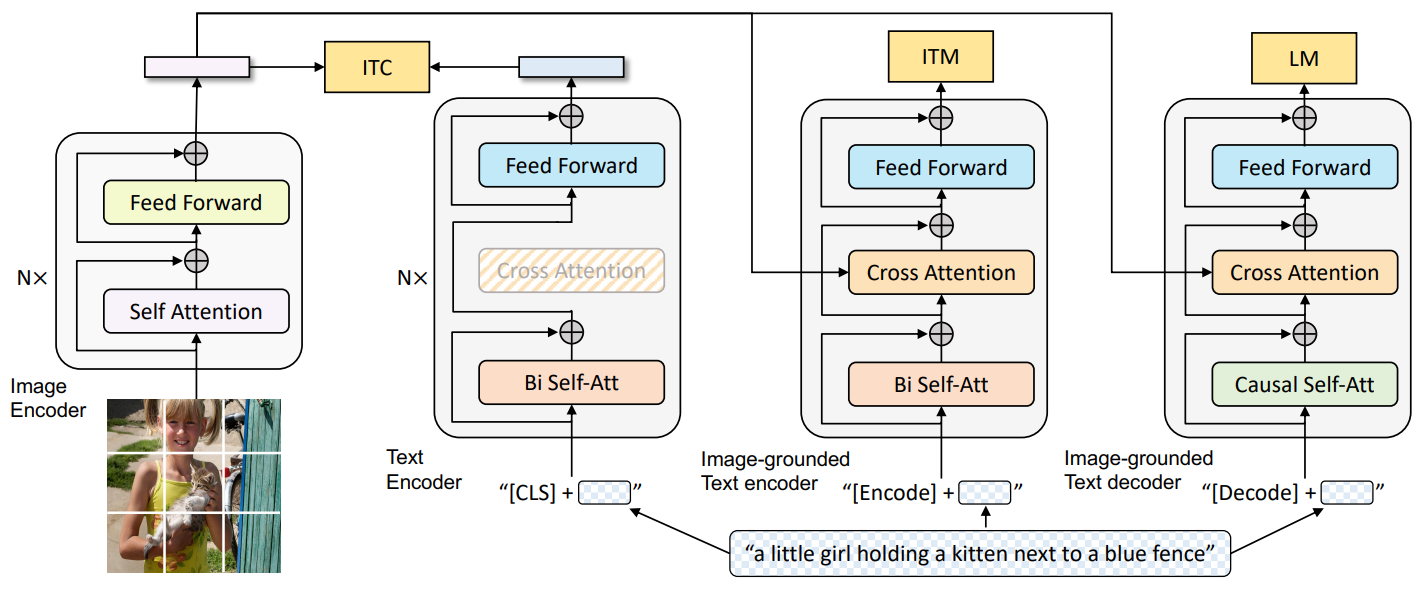
\includegraphics[width=\linewidth]{blip_pretraining.png}
    \caption{BLIP pre-training model architecture: multimodal mixture
of encoder-decoder.}
    \label{fig:blip_pretraining}
\end{figure*}

(1) Unimodal encoders are trained with an image-text contrastive (ITC) loss to align the image and text representations. The image encoder is a visual transformer \cite{dosovitskiy2020image}, which divides an input image into patches and encodes them as a sequence of embeddings. The text encoder is the same as BERT \cite{devlin2018bert}, where a \texttt{[CLS]} token is appended to the beginning of the text input to summarize it.

(2) Image-grounded text encoder is trained with a image-text matching (ITM) loss to distinguish between positive and negative image-text pairs. It has a cross-attention layer between the self-attention layer and the feed forward layer for each transformer block. The output embedding of the \texttt{[Encode]} token is used as the multimodal representation of the image-text pair.

(3) Image-grounded text decoder is trained with a language modeling (LM) loss to generate captions for given images. It replaces the bi-directional self-attention layers in the text encoder with causal self-attention layers. A \texttt{[Decode]} token is used to as the beginning of a sequence.

In order to perform efficient pre-training and improve multi-task learning, the text encoder and text decoder share all parameters except for the self-attention layers. This is enough to capture differences between encoding and decoding tasks.

\subsection{Dataset Bootstraping}

As human-annotated image-text pairs are scarce, vision-language pre-training relies on large-scale image-text pairs automatically collected from the web. However, the texts often do not accurately describe the visual content of the image, making them a noisy supervision. 

To address this, BLIP adds two modules, a captioner and a filter. The learning framework can be seen in Figure \ref{fig:blip_framework}. Both the captioner and the filter are initialized from the same pre-trained MED model, and finetuned individually on the COCO \cite{lin2014microsoft} dataset.

\begin{figure*}[ht]
    \centering
    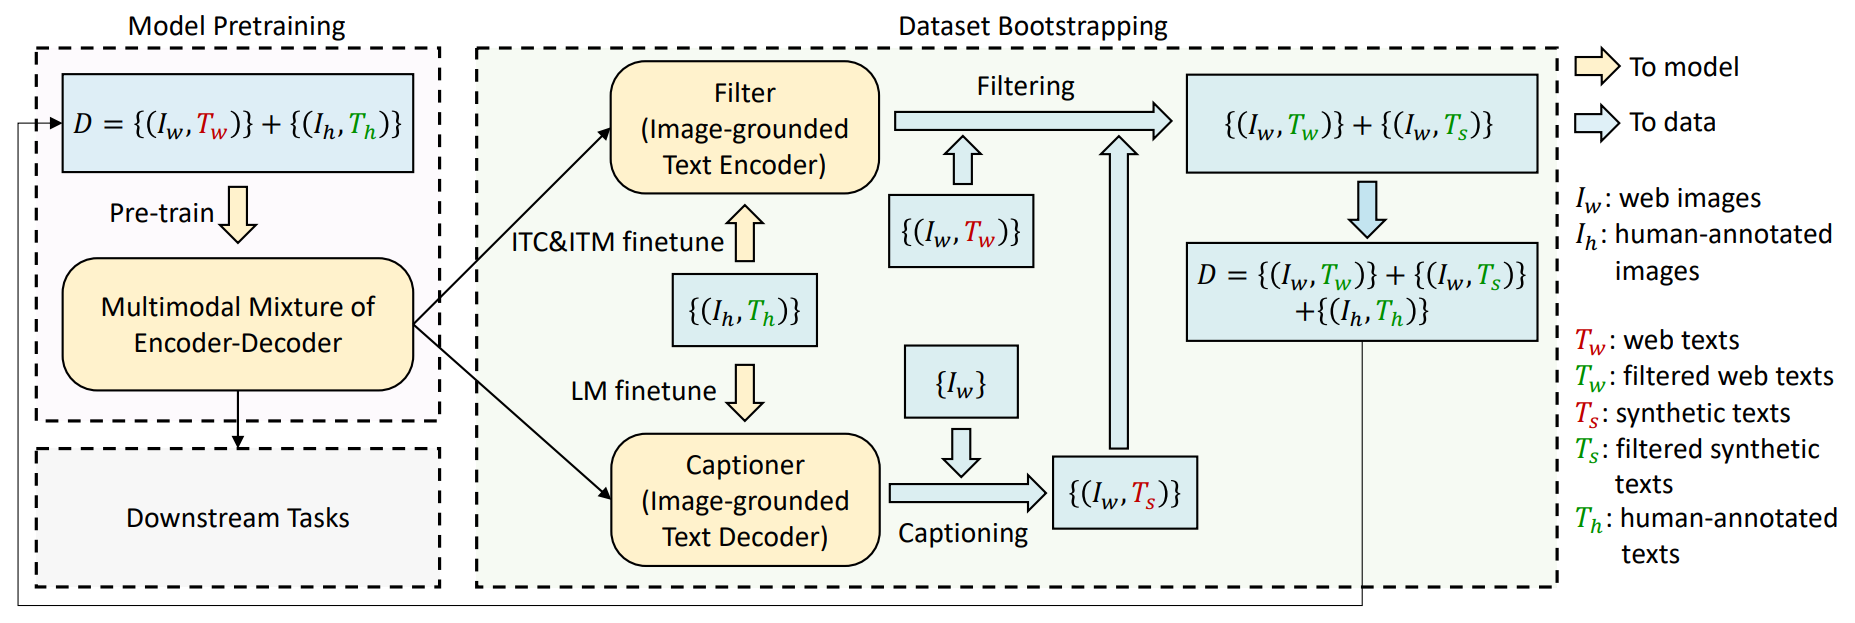
\includegraphics[width=\linewidth]{blip_framework.png}
    \caption{BLIP learning framework: a captioner to produce synthetic captions and a filter to remove noisy captions.}
    \label{fig:blip_framework}
\end{figure*}

The captioner is an image-grounded text decoder. Given the web images, it to generates synthetic captions as additional training samples. The filter is an image-grounded text encoder. It removes noisy captions which do not match their corresponding images. Filtered image-text pairs are combined with the human-annotated pairs to form a new dataset, which is used to pre-train a new model.

\subsection{Finetuning}

On each downstream task, different paths of the pre-trained model are finetuned to achieve different objectives. As the task of our dataset is visual question answering, we will mainly focus on that task.

VQA \cite{antol2015vqa} is a popular vision and language task. Given an image and a question about the image, the task is to provide an accurate answer. VQA\footnote{\url{https://visualqa.org}} dataset is commonly used as a benchmark to evaluate VQA systems. Questions are generally open-ended but multiple choices are provided for some questions. Visual Genome \cite{krishna2017visual} is another popular image-text dataset that was used to finetune the model.

The finetuning architecture for VQA can be seen in Figure \ref{fig:vqa_example}. Image Encoder, Image-grounded Question Encoder and Answer Decoder are used for this task. Encoding questions is similar to encoding the caption related to an image. Decoding an answer is similar to decoding the caption of an image.

\begin{figure*}[ht]
    \centering
    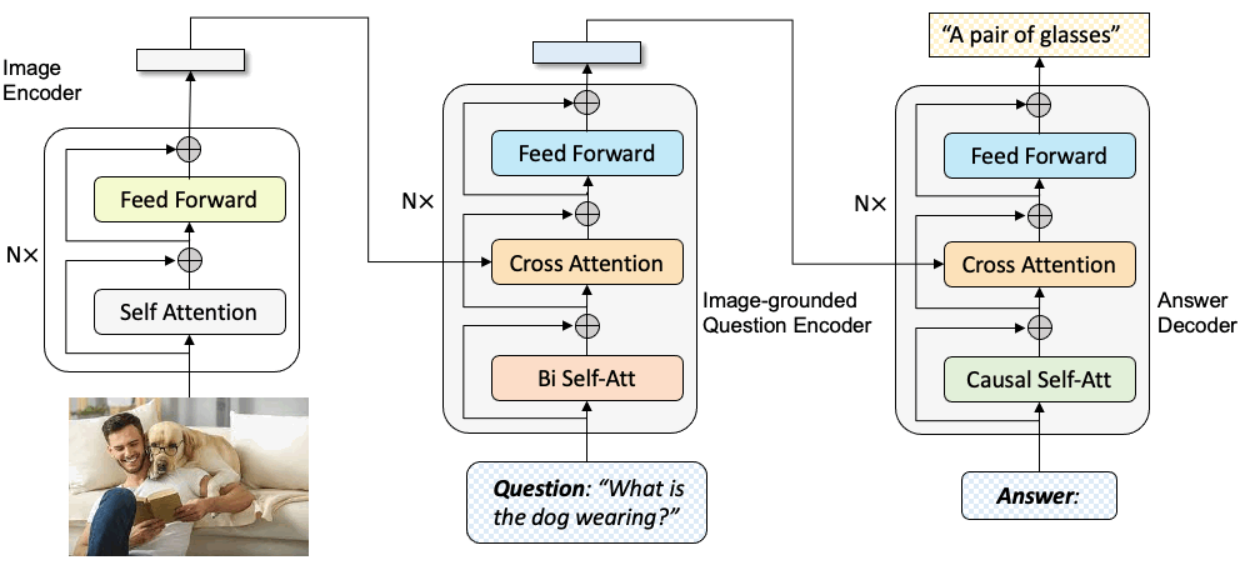
\includegraphics[width=\linewidth]{vqa_example.png}
    \caption{BLIP VQA finetuning architecture.}
    \label{fig:vqa_example}
\end{figure*}

If we compare it to image captioning, VQA requires a more detailed understanding of the image and more complex reasoning \cite{antol2015vqa}. The finetuning architecture for image captioning can be seen in Figure \ref{fig:vqa_example}. The architecture is simpler, only the Image Encoder and Image-grounded Text Decoder are needed.

\begin{figure}[ht]
    \centering
    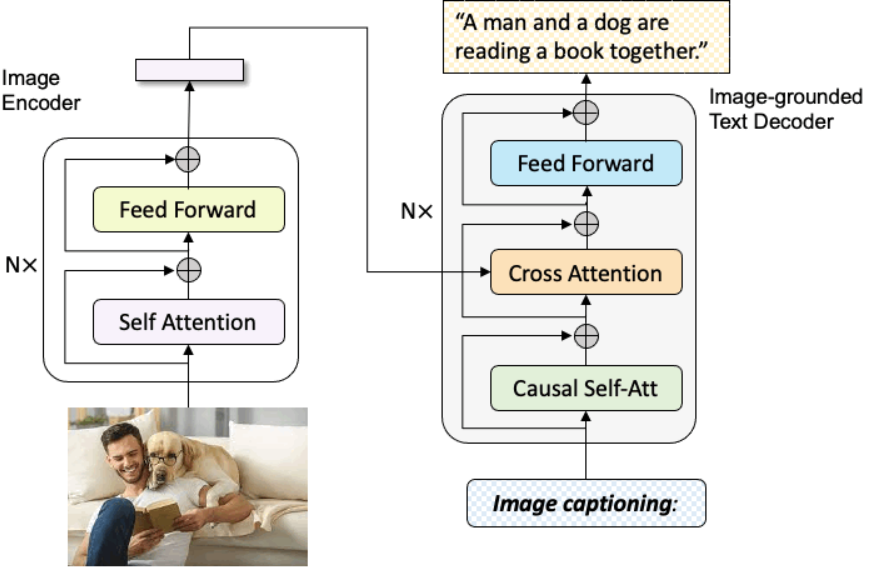
\includegraphics[width=\linewidth]{captioning_example.png}
    \caption{BLIP image captioning finetuning architecture.}
    \label{fig:captioning_example}
\end{figure}

\subsection{Testing}

We test the state-of-the-art BLIP \cite{li2022blip} model on this dataset in a zero-shot setting. This will show the difficulty of each question type and the ability of the model to generalize to different types of images.

Instead of testing the model in a multiple-choice setting, we only take the most probable answer and compare it to the correct one. This makes the questions more difficult for the model. It would be interesting to also test it as multiple-choice and see the differences in results. This could be done by looking at the probabilities that the model assigns to each of the 3 answers, and selecting the one with highest probability.

Another interesting test would be creating more images and questions and finetuning BLIP model on Egunean Behin dataset. This would allow to make a comparison between the VQA dataset and Egunean Behin dataset.

\section{Dataset}

The aim of this dataset is to create visual questions that imitate some questions from Egunean Behin game. These can be used to evaluate models on these types of questions that require understanding visual and language content.

Three types of questions from Egunean Behin game were selected: figures, cubes and maze. There are multiple questions for each image. Questions require counting figures, colors, cubes and understanding the dimensions of the pictures. 

Questions have different levels of difficulty. Figure questions only require counting objects that are visible in the image. Cube questions require more advanced reasoning about objects that are not visible. Maze questions are the most difficult ones, as the model has to understand the maze and find a path.

All the images and questions were generated automatically in two steps. First, we generate as many images as we want. Then, we generate multiple questions for each image. We decided to generate 100 images of each type to test the dataset.

The dataset and code are available at GitHub\footnote{\url{https://github.com/juletx/egunean-behin-vqa}}. Code and data are licensed under GNU General Public License v3.0. The code is based on other works licensed under GNU GPL v3.0 that are mentioned in that repository.

\subsection{Figures}

Images have geometric figures of different types and colors. Figures are selected randomly to create many different images. The size of the figures and axes can be changed to create images with different dimensions and difficulty. 

Images are saved with a name that contains all the necessary data to create questions. The first two digits correspond to dimension of the image. The next digits correspond to the figures in each position of the image. For example, the name of the image in Figure \ref{fig:figures_example} is figures\_6\_4\_417148\_466526\_041585\_724774.png.

\begin{figure}[ht]
    \centering
    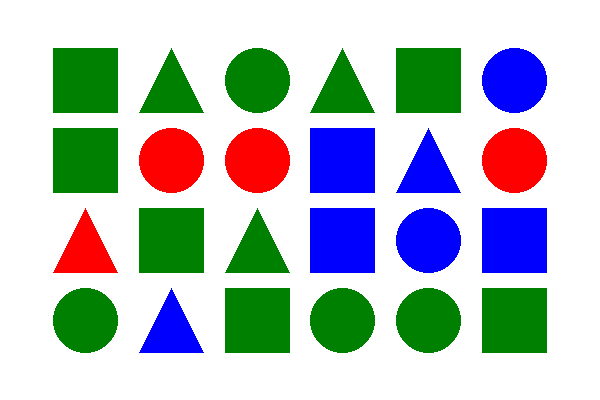
\includegraphics[width=\linewidth]{figures_6_4_417148_466526_041585_724774.png}
    \caption{Figures image example.}
    \label{fig:figures_example}
\end{figure}

18 questions of different types are created for each image. 3 questions about figure, column and row count. 3 questions about figure shape. 3 questions about figure color. 9 questions about figure shape and color combined. Table \ref{tab:figures_example} shows example questions, correct answers (C), wrong answers (W) and BLIP answers (A) for Figure \ref{fig:figures_example}. Most answers of the model are wrong, but many are close to the correct answer.

\begin{table}[ht]
\centering
\begin{tabular}{lllll}
\toprule
Question                  & C       & W     & W & A    \\ \midrule
How many figures?         & 24      & 29     & 26 & 4    \\
How many columns?          & 6       & 4      & 8 & 3     \\
How many rows?            & 4       & 3      & 2 & 3  \\ \midrule
How many triangles?       & 6       & 5      & 8 & 5      \\
How many squares?         & 9       & 7      & 11 & 9     \\
How many circles?         & 9       & 11     & 8 & 9      \\ \midrule
How many red figures?     & 4       & 5      & 3 & 1      \\
How many green figures?   & 13      & 15     & 17 & 3     \\
How many blue figures?    & 7       & 9      & 10 & 1     \\ \midrule
How many red triangles?   & 1       & 3      & 0 & 2      \\ 
How many green triangles? & 3       & 4      & 1 & 3      \\
How many blue triangles?  & 2       & 4      & 1 & 3      \\
How many red squares?     & 0       & 1      & 2 & 1      \\
How many green squares?   & 6       & 4      & 5 & 3      \\
How many blue squares?    & 3       & 5      & 4 & 2      \\
How many red circles?     & 3       & 5      & 4 & 2      \\
How many green circles?   & 4       & 3      & 6 & 3      \\
How many blue circles?    & 2       & 0      & 3 & 3      \\ \bottomrule
\end{tabular}
\caption{Figures questions and answers that correspond to the example image.}
\label{tab:figures_example}
\end{table}

\subsection{Cubes}

Images consist of 3 dimension cubes stack on top of each other. Cubes are stacked on top of each other with the defined probability. Cubes in each layer are colored with the selected colormap. The size of each axis can be controlled to create images with different dimensions. 

Images are saved with a name that contains all the necessary data to create questions. The first three digits correspond to dimension of the image. The next digits correspond to the number of cubes in each position of the image. For example, the name for the image in Figure \ref{fig:cubes_example} is cubes\_4\_4\_3\_0002\_0013\_1133\_3333.png.

\begin{figure}[ht]
    \centering
    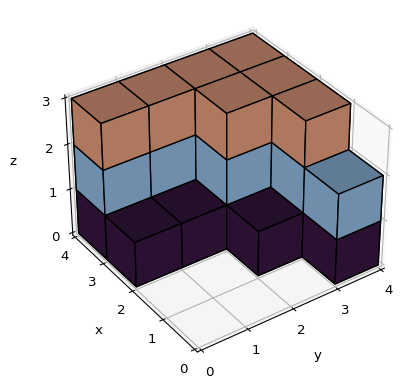
\includegraphics[width=\linewidth]{cubes_4_4_3_0002_0013_1133_3333.png}
    \caption{Cubes image example.}
    \label{fig:cubes_example}
\end{figure}

Many questions of different types are created for each image. The number of questions for each image was 14, but it depends on the dimensions of the images. 3 questions about total, visible and non visible cubes. 4 questions about number of cubes in each x layer. 4 questions about number of cubes in each y layer. 3 questions about number of cubes in each z layer. Table \ref{tab:cubes_example} shows example questions and answers for Figure \ref{fig:cubes_example}. Most answers of the model are wrong and far from the correct answers. This shows that cube questions are more difficult than figure questions.

\begin{table}[ht]
\centering
\begin{tabular}{lllll}
\toprule
Question                     & C       & W     & W & A    \\ \midrule
How many cubes in total?     & 26      & 22     & 21 & 12     \\
How many visible cubes?      & 17      & 16     & 11 & 6     \\
How many non visible?  & 9       & 13     & 10  & 1    \\ \midrule
How many cubes in x 1? & 2       & 0      & 1  & 6     \\
How many cubes in x 2? & 4       & 3      & 6 & 6      \\
How many cubes in x 3? & 8       & 11     & 10 & 6     \\
How many cubes in x 4? & 12      & 15     & 13 & 6     \\ \midrule
How many cubes in y 1? & 4       & 6      & 7  & 4     \\
How many cubes in y 2? & 4       & 3      & 1   & 3    \\
How many cubes in y 3? & 7       & 9      & 8  & 3     \\
How many cubes in y 4? & 11      & 8      & 13 & 3     \\ \midrule
How many cubes in z 1? & 11      & 10     & 12 & 6     \\
How many cubes in z 2? & 8       & 4      & 11 & 6     \\
How many cubes in z 3? & 7       & 11     & 10  & 6    \\ \bottomrule
\end{tabular}
\caption{Cubes questions and answers that correspond to the example image.}
\label{tab:cubes_example}
\end{table}

\subsection{Maze}

A depth-first search algorithm is used to create mazes. The maze consist of a grid of cells and each cell initially has four walls. Starting from a given cell, the aim is to produce a path visiting each cell.

At each step we inspect the neighbouring cells. If any of them have yet to be visited, we pick one and move at random into it by removing the wall between them. If no neighbouring cell is unvisited (a dead end), then backtrack to the last cell with an unvisited neighbour.

After we construct the maze, we have to add a wall so that there is only one possible exit from our starting point. Each edge will have a color so that we can refer to it easier.

The size of the maze can be controlled and We can also select the starting point of the maze. Images are saved with a name that contains all the necessary data to create questions. The first digit corresponds to the index of the image. The next two digits correspond to dimension of the image. The last digits correspond to the starting and ending position. For example, the name for the image in Figure \ref{fig:maze_example} is maze\_0\_12\_8\_0\_2.png.

\begin{figure}[ht]
    \centering
    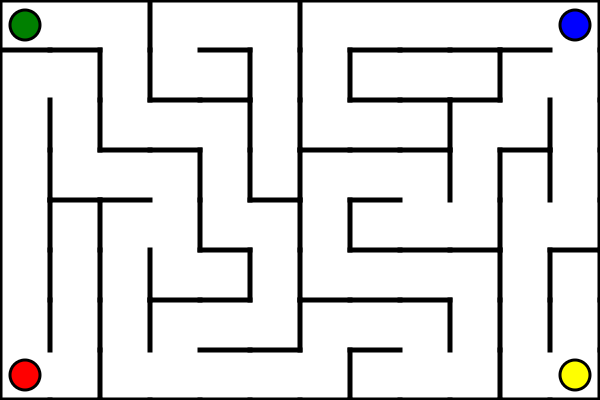
\includegraphics[width=\linewidth]{maze_0_12_8_0_2.png}
    \caption{Maze image example.}
    \label{fig:maze_example}
\end{figure}

Only 4 questions of different types are created for each image. 3 questions about cell, column and row counts. 1 question about maze exit. Table \ref{tab:maze_example} shows example questions and answers for Figure \ref{fig:maze_example}. All the answers are wrong and very far from the correct answer. This shows that these questions are very difficult.

\begin{table}[ht]
\centering
\begin{tabular}{lllll}
\toprule
Question                               & C    & W  & W & A  \\ \midrule
How many cells?                        & 96   & 98  & 87 & 8    \\
How many colums?                       & 12   & 11  & 9 & 0      \\
How many rows?                         & 8    & 7   & 5 & 5     \\ \midrule
Exit from green? & blue & red & yellow & left \\ \bottomrule
\end{tabular}
\caption{Maze questions and answers that correspond to the example image.}
\label{tab:maze_example}
\end{table}

\section{Results}

In this section, we compare BLIP results obtained in VQA finetuting and Egunean Behin zero-shot. BLIP also obtaines great results in many other tasks, but we only focus on the VQAv2.0 dataset. We compare the results obtained in each question type of Egunean Behin dataset.

\subsection{VQA}

BLIP was tested on VQA2.0 dataset \cite{goyal2017making}, which contains a total of 206k images, 1.1M questions and 11M correct answers. Images are divided for training/validation/test in sizes 83k/41k/81k. Both training and validation splits for training, and include additional training samples from Visual Genome. During inference on VQA, the decoder is used to rank the 3,128 candidate answers.

BLIP outperformes previous state-of-the-art methods on VQA as shown in Table \ref{tab:results_vqa}. Using 14M images, BLIP outperforms ALBEF by +1.64\% on the test set. Using 129M images, BLIP achieves better performance than SimVLM, which uses 13× more pre-training data and a larger vision backbone with an additional convolution stage. Best results are achieved when using CapFilt module to filter noisy captions and generate new ones. The difference is not very big in this task, but it is clear that it has a positive impact in the results.

\begin{table}[ht]
\centering
\begin{tabular}{llll}
\toprule
Method        & Images & test-dev & test-std \\ \midrule
LXMERT        & 180K              & 72.42    & 72.54    \\
UNITER        & 4M                & 72.70    & 72.91    \\
VL-T5/BART    & 180K              & -        & 71.3     \\
OSCAR         & 4M                & 73.16    & 73.44    \\
SOHO          & 219K              & 73.25    & 73.47    \\
VILLA         & 4M                & 73.59    & 73.67    \\
UNIMO         & 5.6M              & 75.06    & 75.27    \\
ALBEF         & 14M               & 75.84    & 76.04    \\
SimVLM$_{base}$   & 1.8B              & 77.87    & 78.14    \\ \midrule
BLIP          & 14M               & 77.54    & 77.62    \\
BLIP          & 129M              & 78.24    & 78.17    \\
BLIP$_{CapFilt\-L}$ & 129M              & \textbf{78.25}    & \textbf{78.32}    \\ \bottomrule
\end{tabular}
\caption{Comparison with state-of-the-art methods on VQA.}
\label{tab:results_vqa}
\end{table}

\subsection{Egunean Behin}

We decided to generate 100 images of each type to test the dataset. Each subset creates a different number of questions per image, which results in the counts that can be seen in Table \ref{tab:results_egunean_behin}. There are 300 images and 3600 questions, 3600 correct answers and 7200 wrong answers. Compared to VQA dataset this is a small size, but it is enough to test the performance of the model in a zero-shot setting.

\begin{table}[ht]
\centering
\begin{tabular}{lllll}
\toprule
Subset  & Images & Questions & Acc   & MAE   \\ \midrule
Figures & 100    & 1800      & 16.5  & 3.31  \\
Cubes   & 100    & 1400      & 4.79  & 6.79  \\
Maze    & 100    & 400       & 14.25 & 26.39 \\ \bottomrule
\end{tabular}
\caption{Number of images and questions, accuracy and mean absolute error of BLIP for each subset.}
\label{tab:results_egunean_behin}
\end{table}

As expected, results are very bad compared to VQA dataset with finetuning. The highest accuracy is obtained in the Figures subset, which makes sense because it is the easiest one. Maze also obtains a similar accuracy, but this is due to only having four options in one of the four questions.

As accuracy is an all or nothing metric, it is necessary to calculate mean absolute error to know how close answers are to the correct one. We can see that in this case the error is bigger for the more difficult questions. In the case of figures MAE is 3.31, which means that in average answers were quite close to the correct ones. This is what we noted in the example image.

\section{Conclusions}

Egunean Behin is a new visual question answering dataset based on Egunean Behin game. It consists of three types of questions from the game: figures, cubes and maze. Compared to other datasets that mostly use real-world images, all the artificial images and questions are generated automatically. It can be used to evaluate VQA models in an out-of-domain zero-shot setting.

BLIP is a new VLP framework with state-of-the-art performance on a wide range of downstream vision-language tasks, including both understanding and generation tasks. BLIP pre-trains a multimodal mixture of encoder-decoder model using a dataset bootstrapped from noisy image-text pairs by creating diverse synthetic captions and removing noisy captions.

Great improvements are being made in vision-language tasks such as visual question answering. However, when evaluating in an out-of domain zero-shot setting, we can see that there is still a lot to improve. Future work should also focus on making improvements to the model and data aspects.

Regarding Egunean Behin dataset, many improvements can be made. Images of different sizes could be generated to make questions that are easier or more difficult. More questions could also be added for each image.

Adding more questions types that are present in the game would be great. For example, counting animals, finding words in an alphabet soup and completing puzzles could be added.

It would also be interesting to test BLIP as multiple-choice in this dataset and see the differences in results. Another interesting test would be to create more images and questions and to finetune BLIP model on Egunean Behin dataset. Testing other models to see the differences would also be an interesting experiment.

\bibliography{egunean_behin_vqa}
\bibliographystyle{acl_natbib}

\end{document}
